% It’s Time to Learn drawing Petri Nets in TikZ!
% Four Season Petri Nets in TikZ
% Latexdraw.com
% 17/02/2021, 23:00

\documentclass[border = 0.2cm]{standalone}
\usepackage{tikz}

\usetikzlibrary{positioning,petri,arrows.meta}

\begin{document}

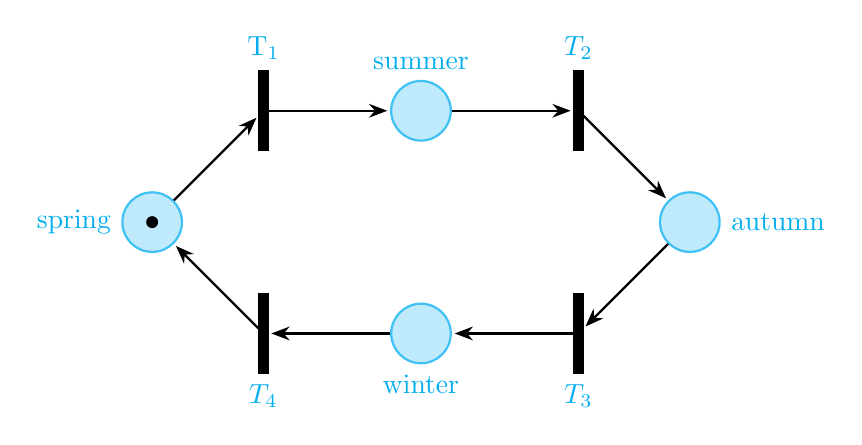
\begin{tikzpicture}[
% Change style
	thick,
	node distance=2cm,
	on grid,
	pre/.style={<-, shorten <=1pt, >={Stealth}},
	post/.style={->,shorten >=1pt, >={Stealth}},
	every transition/.style={fill,minimum width=1mm, minimum height=10mm},
	every place/.style={fill=cyan!25,draw=cyan!75},
	every label/.style={cyan}]

% Place 1
\node[place,tokens=1,
	label=left:spring] (place1) {};

% Transition 1
\node[transition, above right= of place1,
	label=above:T$_1$] (trans1) {};

% Transition 4
\node[transition,below right= of place1,
	label=below:$T_4$] (trans4) {}; 

% Place 2
\node[place,right=of trans1,
	label=above:summer] (place2) {};

% Transition 2
\node[transition,right= of place2,
	label=above:$T_2$] (trans2) {};

% Place 3
\node[place,below right=of trans2,
	label=right:autumn] (place3) {};

% Place 4
\node[place,right=of trans4,
	label=below:winter] (place4) {};

% Transition 3
\node[transition,right= of place4,
	label=below:$T_3$] (trans3) {};

% Connections
\draw (place1) edge[post] (trans1)
	(trans1) edge[post] (place2) 
	(place2) edge[post] (trans2)
	(trans2) edge[post] (place3)
	(place3) edge[post] (trans3)
	(trans3) edge[post] (place4)
	(place4) edge[post] (trans4)  
	(trans4) edge[post] (place1);

\end{tikzpicture}

\end{document}